% Ubah judul dan label berikut sesuai dengan yang diinginkan.
\section{ARCHITECTURE}
\label{sec:arsitektur}

\subsection{System Architecture}
\begin{figure}[H] \centering
  % Nama dari file gambar yang diinputkan
  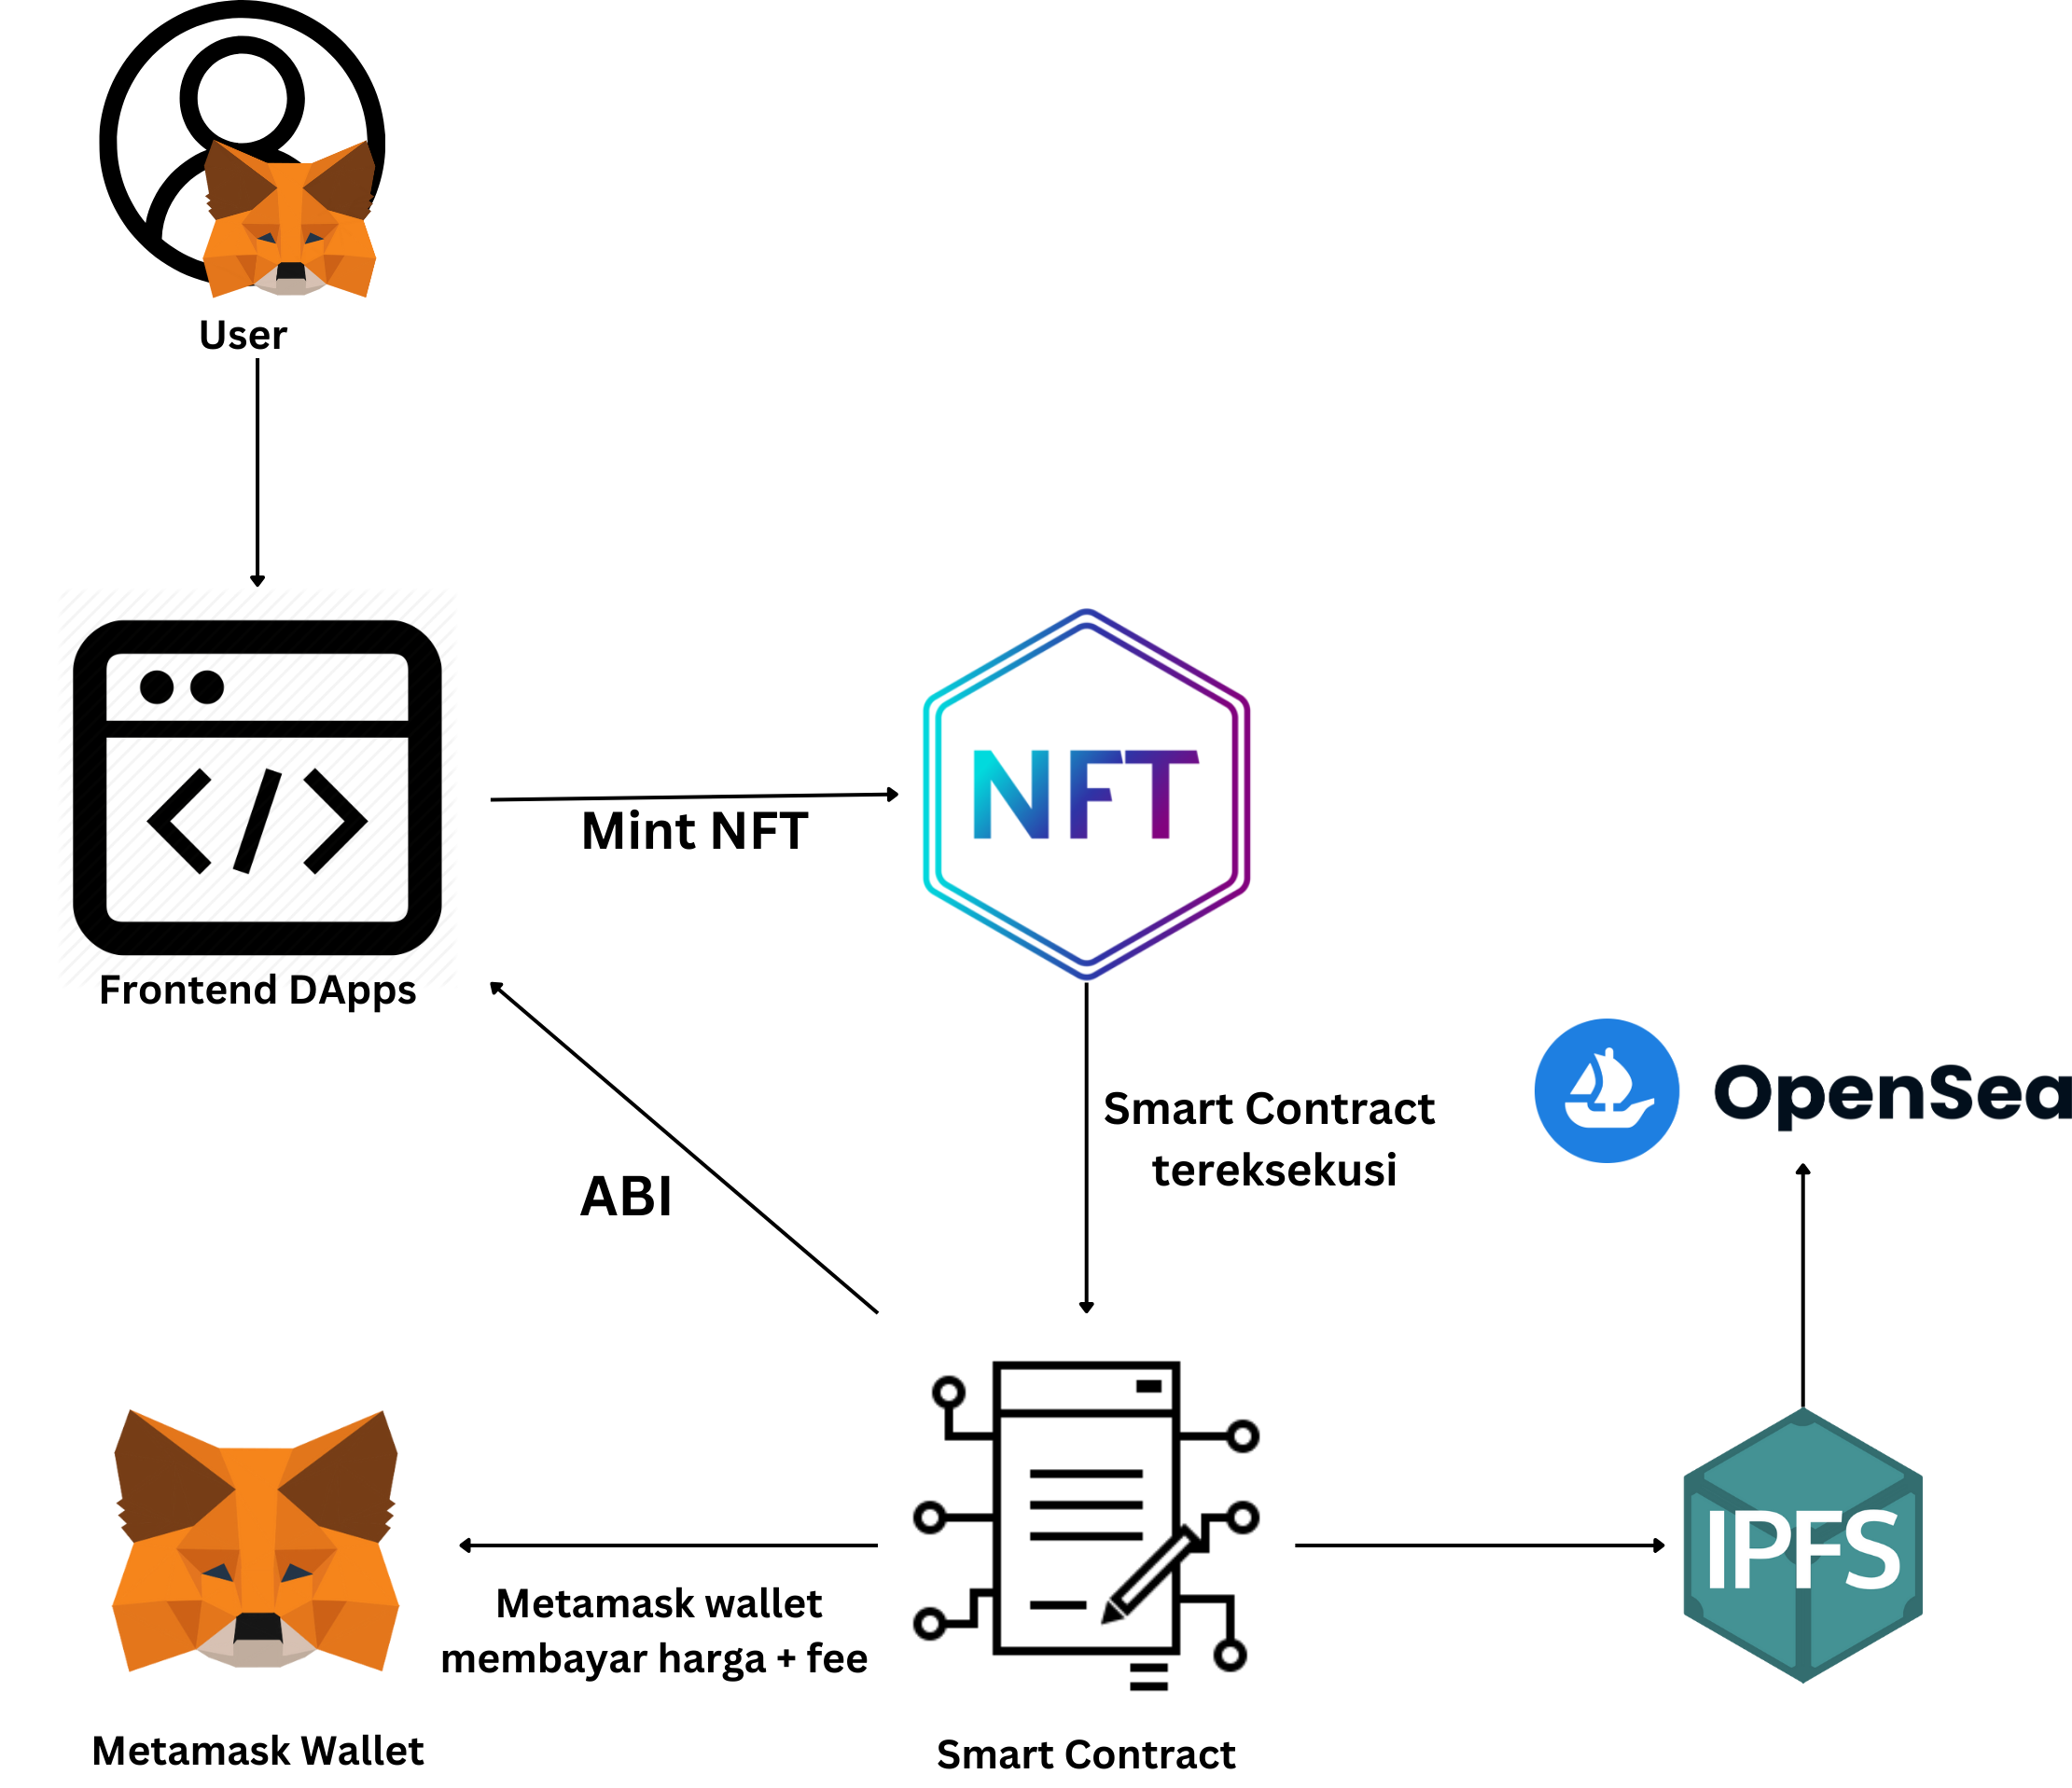
\includegraphics[scale=0.14]{gambar/desain_sistem_new.png}
  % Keterangan gambar yang diinputkan
  \caption{Desain sistem}
  % Label referensi dari gambar yang diinputkan
  \label{fig:desain_sistem}
\end{figure}

In the development of this smart contract system to function as intended by the author for completing this thesis, the author has designed a system architecture. In this system architecture, there is a role for the user who can become the owner of a token, and the user is the party with limited access to a token within a specified time. There is also a front end for the minting process of NFT tokens. To access the front end, both the owner and the user must connect using a Metamask wallet to interact.

% On the front end, it connects with the smart contract when a user performs Minting, where the process involves the user uploading a digital asset they own to IPFS through a backend application, which then returns a Content Identifier (CID). A CID is a file address within IPFS used to access that file. The obtained CID is then uploaded to the blockchain network and becomes a token. Data about the available NFTs can be directly accessed by the front end through the smart contract on the blockchain.

% \vspace{0.5 cm}

\subsection{Minting Process}
\begin{figure}[H] \centering
  % Nama dari file gambar yang diinputkan
  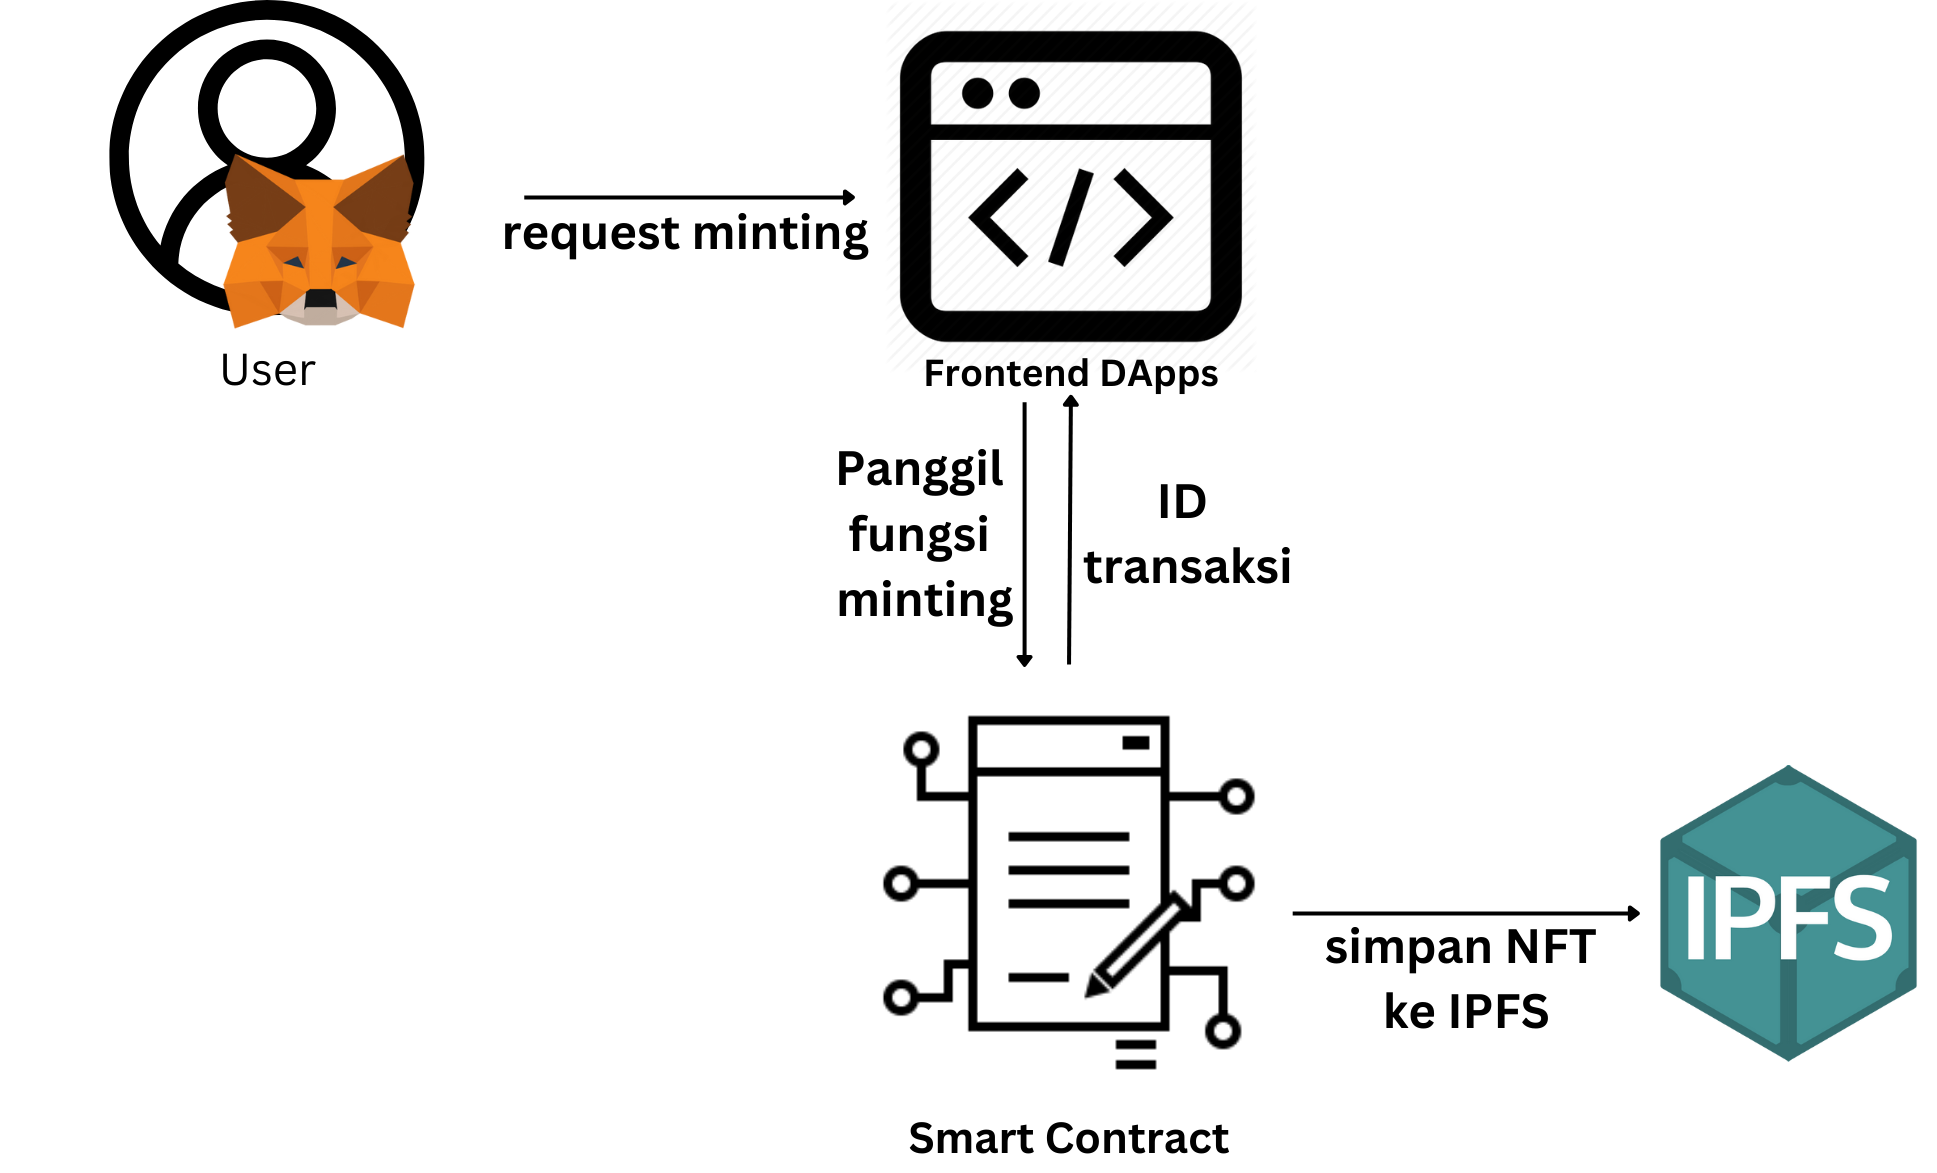
\includegraphics[scale=0.17]{gambar/proses_minting.png}
  % Keterangan gambar yang diinputkan
  \caption{Desain sistem}
  % Label referensi dari gambar yang diinputkan
  \label{fig:proses_minting}
\end{figure}

The minting process is the initial step where a new NFT is created on a platform. During this process, various important details about the NFT must be defined, including its name, description, category, available supply, and the visual asset representing the NFT, which could be a 2D image, 3D model, or video. The initial price, the collection that includes the NFT, and other attributes must also be determined. Once the minting process is complete, the data from the newly created NFT is stored in the InterPlanetary File System (IPFS), which allows for decentralized storage and access to data. This storage ensures that all related information, such as ownership recorded in the NFT’s attributes, can be accessed permanently and securely.

\subsection{Methods}
\begin{figure}[H] \centering
  % Nama dari file gambar yang diinputkan
  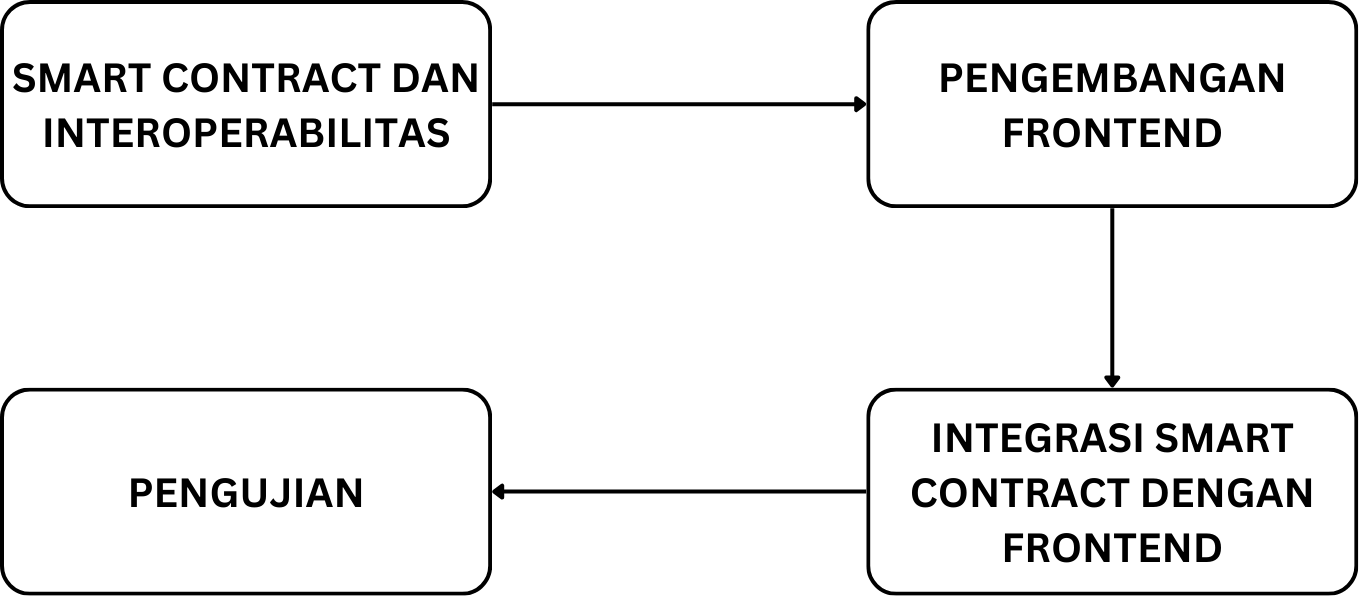
\includegraphics[scale=0.20]{gambar/metodologi_new.png}
  % Keterangan gambar yang diinputkan
  \caption{Metodologi Pengerjaan}
  % Label referensi dari gambar yang diinputkan
  \label{fig:metodologi}
\end{figure}

\subsubsection{Smart Contract and Interoperability}
In this stage, the author develops a smart contract system used for creating interoperable tokens using the Solidity programming language. This smart contract system acts as a bridge to process requests generated from user interactions on the frontend to the blockchain network. Upon compiling the smart contract, an Application Binary Interface (ABI) is generated, which can be used on the frontend for encoding and decoding data, allowing the frontend application to send precise instructions to the smart contract and understand the data returned by it. The smart contract developed by the author includes several core functions for the developed token.

\subsubsection{Frontend Development} 
To integrate a React application with the Ethereum blockchain, we utilize two primary libraries: ethers.js and web3.js. These libraries provide the necessary functionality to interact with the Ethereum blockchain, though they approach it slightly differently. Ethers.js is known for its minimalistic API and ease of use, which is particularly suitable for projects with simpler needs and a focus on reading and writing data to the blockchain. This library offers powerful functions for interacting with smart contracts, such as sending transactions, reading contract statuses, and handling event notifications.

\subsubsection{Integrating Smart Contract with Frontend}
This stage enables applications built with React.js to interact directly with smart contracts deployed on the Ethereum network. To achieve this integration, we use the ethers.js library, which provides a clean and user-friendly interface for communicating with Ethereum.

% Once the smart contract is developed and deployed, the ABI (Application Binary Interface) of the contract is used to construct a contract instance within the React application. The ABI allows the frontend to understand what functions are available in the smart contract, including the variables and data types used. With this information, ethers.js can invoke these functions, such as safeMint or transferOwnership, according to the logic defined in the contract.

\subsubsection{Testing}
This stage includes several steps for testing the smart contract, namely unit testing and integration testing.

% \begin{itemize}
%     \item Unit Testing
%     This testing focuses on validating each component individually. In the context of a React.js frontend, this means testing components separately to ensure that they behave as expected. Unit testing is also conducted on the smart contract functions to verify their business logic, such as minting or token transfer functions. This testing is typically performed using the React framework for frontend and Hardhat for smart contracts.

%     \item Integration Testing
%     Following unit testing, the next step is integration testing, which ensures that all components in the application work well when combined. In the context of smart contract integration, this involves testing the interaction between the React.js frontend and the smart contract through ethers.js or web3.js. Integration testing helps detect issues in the data flow between the frontend and blockchain, including transaction validation and correct state updates.
% \end{itemize}

% \subsection{Tools Used}
% \subsubsection{Solidity}
% Solidity is a high-level programming language specifically designed for developing smart contracts on the Ethereum blockchain platform. This language offers syntax optimized for handling smart contract operations, including support for variables, functions, and complex control structures, all crucial for creating efficient and secure decentralized applications. Additionally, Solidity includes various security features that prevent common vulnerabilities such as reentrancy attacks and overflows. A major advantage of Solidity is its ability to run on the Ethereum Virtual Machine (EVM), a runtime environment that makes it compatible with various types of blockchains that adopt the EVM standard. Using Solidity opens opportunities for developers to implement complex contract logic that can interact directly with the blockchain, providing a high level of transparency and reliability in digital transactions.

% \subsubsection{Metamask}
% MetaMask is a digital wallet specifically designed to facilitate users in managing crypto assets like Ether (ETH) and interacting with decentralized applications (dApps) on the Ethereum network. Its function extends beyond just storing and managing crypto; it also acts as a bridge connecting users to the Ethereum ecosystem. Available as a browser extension, MetaMask allows users to execute crypto transactions directly from their web browser without the need for additional software. MetaMask also supports other Ethereum-compatible blockchain networks, enabling users to participate in a variety of blockchain activities such as blockchain-based games, digital art markets, and decentralized finance (DeFi) platforms. With MetaMask, users can seamlessly switch between these networks, exploring the crypto world more securely and conveniently.

% \subsubsection{Hardhat}
% Hardhat is a development framework specifically designed to facilitate the development, testing, and deployment of \emph{smart contracts}. This tool provides a range of features that allow blockchain developers to work more efficiently. With Hardhat, developers can run a local Ethereum environment that simplifies the process of testing and debugging. Hardhat supports complex automation tasks and integrates a broad software stack, including customizable plugins and scripts to enhance functionality and efficiency. This framework also facilitates smoother interactions with the public Ethereum networks and testnets, allowing developers to receive quick and effective feedback on how their \emph{smart contracts} perform under actual network conditions.

% \subsubsection{InterPlanetary File System}
% The InterPlanetary File System (IPFS) is a distributed hypermedia protocol aimed at making the web faster, safer, and more open. It has become increasingly popular among developers, especially for developing smart contracts for Non-Fungible Tokens (NFTs). Essentially, IPFS enables the storage and sharing of data in a distributed network, similar to a peer-to-peer system. Each file and all its blocks are given a unique cryptographic hash, serving as a unique address on the network.

% In the context of NFTs, IPFS is particularly useful as it offers a solution to the dependence on a single server or storage location, which could be a point of failure. For example, if the metadata or digital assets of an NFT, such as images, videos, or audio files, are stored only on a centralized server, there's a risk that the data could be lost or deleted. By using IPFS, these files are stored across multiple nodes in the network, enhancing data resilience and availability. Whenever a file is requested, IPFS retrieves bits of it from multiple nodes, rather than pulling the entire file from a single location, speeding up load times and reducing the load on the network.

% \subsubsection{React.js}
% React.js is a popular and powerful JavaScript library for building user interfaces, commonly known as UIs. The strength of React.js lies in its ability to efficiently and effectively construct dynamic web applications. It enables developers to create large and complex UI components that can be well-managed through the use of state and props, providing a way for efficient data flow and re-rendering.

% Using React.js, developers can leverage libraries such as Web3.js or Ethers.js to interact directly with the Ethereum blockchain, where smart contracts are deployed. This allows applications to query and update the blockchain transparently, displaying information such as NFT ownership, transaction history, and NFT metadata in real-time.

% \subsubsection{Web3.js}
% Web3.js is a crucial JavaScript library for developing web applications that interact with the Ethereum blockchain, particularly within the Web 3.0 ecosystem. This library allows frontend developers to directly communicate with Ethereum nodes, leveraging blockchain functionalities such as smart contracts, transactions, and account management directly from a user's browser.

% Integrating Web3.js into React.js applications enables developers to utilize React hooks and components to react to blockchain state changes in real-time. This includes updates on balances, transaction statuses, and modifications to smart contract data. Such functionality enhances the user experience by providing a consistent and up-to-date view of the blockchain's status, which is crucial in applications demanding high reliability and transparency.

% \subsubsection{Ethers.js}

% Ethers.js is a lightweight JavaScript library designed to interact with the Ethereum blockchain. It is particularly well-suited for frontend application development with React.js due to its simple and modular API, which facilitates the efficient development of decentralized applications (DApps). Ethers.js provides essential functions such as connecting to user wallets, creating and sending transactions, and interacting with smart contracts.

% In development with React.js, Ethers.js aids in integrating blockchain functions into React components cleanly and effectively. For example, by using React hooks like useState and useEffect, developers can seamlessly integrate the status of the Ethereum blockchain into the application's UI, updating the UI in real-time as changes occur on the blockchain such as transaction confirmations or updates to contract data.

% \subsubsection{Etherscan}
% Etherscan is a web-based analytics platform that allows users to track Ethereum transactions, smart contracts, and blockchain status in real-time. This platform provides detailed insights into all activities occurring on the Ethereum network, including information on the latest blocks, ongoing transactions, and circulating tokens. Etherscan is also widely used by developers to check and verify the source code of smart contracts, which is a crucial aspect in ensuring transparency and security within the Ethereum ecosystem. With its user-friendly interface, Etherscan has become an essential tool for anyone involved in the Ethereum blockchain industry to monitor, verify, and analyze transactions and contracts.

% \subsubsection{Token ERC-721}
% ERC-721 is a standard for representing non-fungible assets (NFTs) on the Ethereum blockchain. This standard allows for the unique representation of digital assets such as artwork, collectibles, and in-game items in the form of digital tokens. Each ERC-721 token possesses a unique identifier and can have associated metadata, distinguishing it from other tokens on the blockchain. This feature facilitates the creation, trading, and selling of digital assets in a decentralized and transparent manner. ERC-721 also supports functions that allow token owners to transfer, approve, or access information regarding token ownership, which is crucial for applications in the Web3 ecosystem and the digital economy.
